\subsection{Data Modeling and Article Extraction}
The first phase in the program consists in parsing the article streams and producing the data structures needed in the subsequent steps. Though conceptually simple, the parsing has been challenged by several practical constraints. We will first give an overview of the data generated in this phase, and then a more technical description of the processing steps. Lastly, we will describe the practical problems we encountered and how we dealt with them.

\subsubsection{Parser output overview}
The articles stream we were provided spanned around two centuries of article issues. During such a long period, the French language has been subject to a progressive drift. In a way, the streams are composed of slightly different idioms which belong to particular temporal slices. Typically, a word like "Internet" only appears in the later part of the streams. In our project, this could potentially create a bias because of the background model, a structure described below. In order to compensate this, the program will not analyze the entire dataset, but a temporal subset which we define as the \emph{time frame}. Consequently, from the program's "perspective", the time frame acts as the dataset, so we will use this term instead when there is no ambiguity.
The \emph{background model} is an unique object on the whole dataset (i.e time frame). It allows to retrieve the distribution of every distinct word in the dataset. This structure is used during the theme analysis to determine how common a word is.
For the next part, we will differentiate two different phases in the processing pipeline: the theme extraction, where we perform the Expectation-Maximization (EM) algorithm, and the theme "strength" analysis, which uses the Hidden Markov Models (HMM). For the EM phase, the parser has to provide a structure containing the word count inside each individual article text. For that, we use an object representing a "parsed" article, which contains the count of each distinct word in this article, as well as some other properties (issue date, stream identifier...). These parsed articles must be grouped by small sub-partitions of the time frame. Effectively, the EM part receives an RDD of time partitions containing a small part of the parsed articles. The HMM part requires the chronological concatenation of all the words in the dataset, where a timestamp is attributed to each word. In order to reduce the memory and CPU usage of such a structure, we don't store the words as Java String objects; rather, we first associate each distinct word to a unique integer identifier, and then produce the word concatenation as an ordered RDD of integers. Both the EM and HMM parts need to access the background model.

\subsubsection{Data processing pipeline}
The parser does not produce all its output in one single run. The background model must be computed at the beginning, but the input provided for the EM and HMM parts are generated "on demand", in order to avoid storing pending data (we don't want to keep the HMM input for the whole program, only to use it once at the end). However, it would be expensive to parse and transform the XML files from scratch at each of these steps. Instead, we will produce an intermediary RDD from which all these outputs can be derived. First, we parse the XML streams, retrieve the articles, and segment their text content into a list of words. This list, along with other informations about the article like the issue date and the title, are stored in a container we named "segmented article", which is accumulated in our base RDD.
The background model is generated immediately after this base RDD is finished, simply by counting the number of occurrences of each distinct word, and then associating each word to the ratio of its individual number of occurrences to the total amount of words in the dataset.
In a similar way, we generate the EM phase input by associating each word to its number of occurrences inside every segmented article individually. Using a provided partitioning of the time frame into time partitions, the parser returns the RDD of grouped parsed articles.
Finally, for the HMM phase, we first use the background model to build a lexicon that translates each unique word into an integer identifier. The segmented articles are then sorted chronologically, after what we extract their lists of words, translate them into lists of identifiers using the lexicon, and assemble all the results in one single RDD.
It is noticeable that these operations are quite redundant. Part of this problem is due to the fact that we are exposed to a "chicken-and-egg" situation; the background model must be produced from the list of extracted articles, but we also need the background model during the processing of the article RDDs (and not only for the HMM phase as we will see in the next section). Because of this, and other optimizations that we describe below, we inevitably apply similar transformations over the whole dataset. Nevertheless, all of the operations are particularly simple and can be fully parallelized, resulting in a satisfying total execution time.

\begin{figure}[b]
   \caption{\label{parser_processing_steps} Parser processing pipeline}
   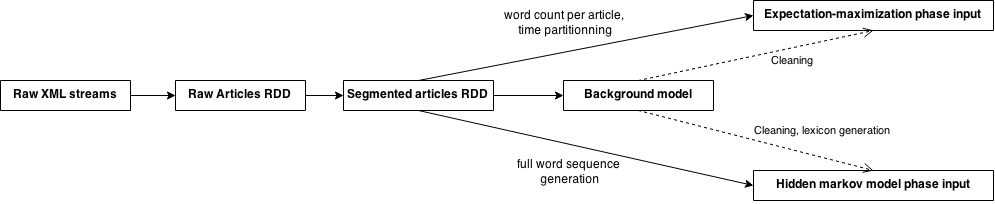
\includegraphics{parser_processing_steps.png}
\end{figure}